% Appendix additions prepared from train-only aggregate sources.
% Source bindings and scope: appendix_evidence.json and appendix_evidence.md.
\section{Data definitions and training distributions}
\label{app:data-characteristics}
Taxi events record pickup counts in active spatial-cell hours. Intermittent
events contain positive site--part order quantities, and RAF events contain
positive monthly spare-parts demands. Instacart aggregates product rows for
each user on the same recorded activity day, so its quantity measures basket
size rather than physical units. Empty calendar periods extend the interval
between events instead of creating zero-quantity targets. The recorded units
are hours, weeks, months, and days, respectively. Instacart intervals are
top-coded at 30 days.

Table~\ref{tab:train-characteristics} describes the frozen training
populations. Quantity summaries include every training event, whereas gap
and usable-history summaries exclude each series' first event because it
has no predecessor for prediction. Quantiles select the nearest observed
value. Each summary weights events or prediction targets equally within
its population, rather than weighting series equally.

Usable history counts the observed predecessor events retained for a target
after both window restrictions. The inclusive recorded-time window ends at
the last observed event. Appending the target before sequence truncation
reserves one position for it, so at most the sequence cap minus one observed
events remain. Neither the target nor padding contributes to usable history.
Table~\ref{tab:data} specifies the windows and caps. The train descriptions
therefore characterize the same input contract across the MLP and CNN+GRU
studies, although those architectures process the retained events differently.

\begin{table}[t]
\caption{Training-only event characteristics. Quantity summaries include all
training events; gap, usable-history, and adjacent-pair summaries describe
targets after excluding the first event of each series. Correlation is
defined in Appendix~\ref{app:lag}.}
\label{tab:train-characteristics}
\centering\scriptsize
\setlength{\tabcolsep}{4pt}
\begin{tabular}{@{}lrrrr@{}}
\toprule
Characteristic & Taxi & Intermittent & RAF & Instacart\\
\midrule
Time unit & Hour & Week & Month & Day\\
Training series & 131 & 5,000 & 5,000 & 206,209\\
Training event rows & 38,524 & 398,824 & 30,779 & 2,197,401\\
Training targets & 38,393 & 393,824 & 25,779 & 1,991,192\\
Quantity: median & 7 & 2 & 2 & 8\\
Quantity: 95th percentile & 1,562 & 46 & 60 & 25\\
Quantity: 99th percentile & 3,449 & 187 & 200 & 35\\
Quantity: maximum & 6,322 & 477 & 2,062 & 175\\
Recorded gap: median & 1 & 3 & 6 & 7\\
Recorded gap: 95th percentile & 5 & 5 & 23 & 30\\
Usable history: median & 129 & 40 & 3 & 5\\
Usable history: 95th percentile & 168 & 144 & 8 & 14\\
History $\leq7$ events (\%) & 2.41 & 8.89 & 93.58 & 72.13\\
Within-series log correlation & 0.749 & 0.928 & -0.105 & 0.037\\
Equal adjacent quantities (\%) & 20.33 & 61.99 & 33.30 & 10.24\\
\bottomrule
\end{tabular}
\end{table}

\begin{figure}[t]
\centering
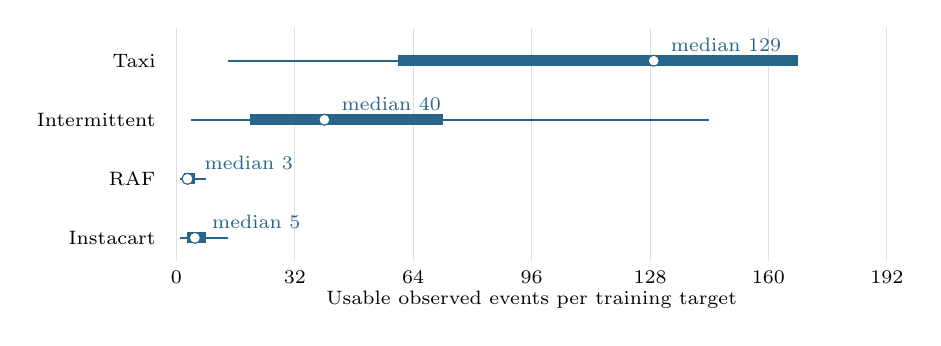
\begin{tikzpicture}[x=.047cm,y=.75cm,font=\scriptsize]
\definecolor{profileblue}{RGB}{40,101,138}
\draw[gray!25] (0,-.4)--(0,3.55);
\node[below] at (0,-.4) {0};
\draw[gray!25] (32,-.4)--(32,3.55);
\node[below] at (32,-.4) {32};
\draw[gray!25] (64,-.4)--(64,3.55);
\node[below] at (64,-.4) {64};
\draw[gray!25] (96,-.4)--(96,3.55);
\node[below] at (96,-.4) {96};
\draw[gray!25] (128,-.4)--(128,3.55);
\node[below] at (128,-.4) {128};
\draw[gray!25] (160,-.4)--(160,3.55);
\node[below] at (160,-.4) {160};
\draw[gray!25] (192,-.4)--(192,3.55);
\node[below] at (192,-.4) {192};
\node[anchor=east] at (-3,3) {Taxi};
\draw[profileblue,line width=.6pt] (14.0,3)--(168.0,3);
\draw[profileblue,line width=4pt] (60.0,3)--(168.0,3);
\filldraw[draw=profileblue,fill=white] (129.0,3) circle[radius=2pt];
\node[anchor=west,text=profileblue] at (131.0,3.27) {median 129};
\node[anchor=east] at (-3,2) {Intermittent};
\draw[profileblue,line width=.6pt] (4.0,2)--(144.0,2);
\draw[profileblue,line width=4pt] (20.0,2)--(72.0,2);
\filldraw[draw=profileblue,fill=white] (40.0,2) circle[radius=2pt];
\node[anchor=west,text=profileblue] at (42.0,2.27) {median 40};
\node[anchor=east] at (-3,1) {RAF};
\draw[profileblue,line width=.6pt] (1.0,1)--(8.0,1);
\draw[profileblue,line width=4pt] (2.0,1)--(5.0,1);
\filldraw[draw=profileblue,fill=white] (3.0,1) circle[radius=2pt];
\node[anchor=west,text=profileblue] at (5.0,1.27) {median 3};
\node[anchor=east] at (-3,0) {Instacart};
\draw[profileblue,line width=.6pt] (1.0,0)--(14.0,0);
\draw[profileblue,line width=4pt] (3.0,0)--(8.0,0);
\filldraw[draw=profileblue,fill=white] (5.0,0) circle[radius=2pt];
\node[anchor=west,text=profileblue] at (7.0,0.27) {median 5};
\node at (96,-1.05) {Usable observed events per training target};
\end{tikzpicture}
\caption{Available training history under the frozen input windows. Thin
lines span the 5th--95th percentiles, thick lines the 25th--75th percentiles,
and circles mark medians. These target-weighted distributions characterize
input availability, not model performance.}
\label{fig:train-history}
\Description{Training-history distributions for four datasets. Taxi and
Intermittent supply longer observed histories than RAF and Instacart.}
\end{figure}

Figure~\ref{fig:train-history} indicates substantial differences in available
history. The median spans 129 observed events on Taxi and 40 on Intermittent,
compared with three on RAF and five on Instacart. Thus an equal nominal
sequence cap would not imply equal evidence per prediction. These training
distributions describe the input populations; they neither measure which
events a trained model retains nor determine its forecasting error.

\section{Event-lag association in the training data}
\label{app:lag}
For series $e$ and event lag $\ell$, pair
$x^{(\ell)}_{e,j}=\log(1+q_{e,j-\ell})$ with
$y^{(\ell)}_{e,j}=\log(1+q_{e,j})$ whenever both events belong to that
training series. Each lag counts observed events in sequence order.
It does not denote elapsed calendar time. The descriptive calculation
includes the complete training sequence, without the model's recorded-time
window or sequence-length cap.

Let $\bar x_e^{(\ell)}$ and $\bar y_e^{(\ell)}$ be the separate means
of the predecessor and successor members of those pairs. The statistic is
\begin{equation}
 r_{\ell}=\operatorname{Corr}\!\left(
 x^{(\ell)}_{e,j}-\bar x_e^{(\ell)},\,
 y^{(\ell)}_{e,j}-\bar y_e^{(\ell)}\right),
 \label{eq:train-lag-correlation}
\end{equation}
where correlation pools the centered pairs across series. Centering removes
between-series differences in mean log quantity, but each pair still
contributes to the pooled sums. This statistic is consequently different
from an average of series-specific correlations. The lag-one column
corresponds to the adjacent log correlation in
Table~\ref{tab:train-characteristics}.
% Generated from reports/titantpp_train_lag_heatmap_20261002_v1/analysis.json.
\begin{figure}[t]
\centering
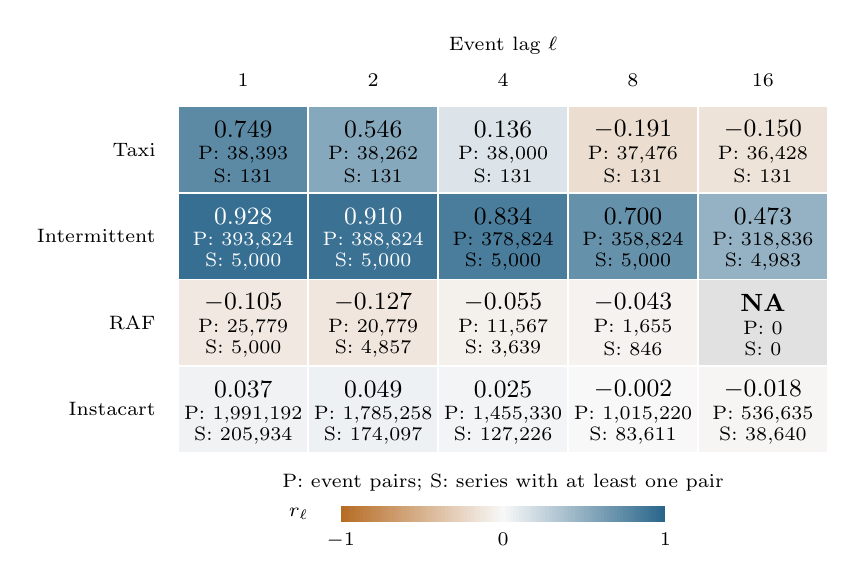
\begin{tikzpicture}[x=1.65cm,y=1.10cm,font=\scriptsize]
\node at (2.5,4.70) {Event lag $\ell$};
\node at (0.5,4.30) {1};
\node at (1.5,4.30) {2};
\node at (2.5,4.30) {4};
\node at (3.5,4.30) {8};
\node at (4.5,4.30) {16};
\node[anchor=east] at (-.10,3.5) {Taxi};
\definecolor{lagcell00}{HTML}{5C8AA5}
\filldraw[fill=lagcell00,draw=white,line width=.6pt] (0,3) rectangle (1,4);
\node[text=black,font=\bfseries\small] at (0.5,3.73) {$0.749$};
\node[text=black,font=\scriptsize] at (0.5,3.44) {P: 38,393};
\node[text=black,font=\scriptsize] at (0.5,3.20) {S: 131};
\definecolor{lagcell01}{HTML}{86A8BC}
\filldraw[fill=lagcell01,draw=white,line width=.6pt] (1,3) rectangle (2,4);
\node[text=black,font=\bfseries\small] at (1.5,3.73) {$0.546$};
\node[text=black,font=\scriptsize] at (1.5,3.44) {P: 38,262};
\node[text=black,font=\scriptsize] at (1.5,3.20) {S: 131};
\definecolor{lagcell02}{HTML}{DCE4E9}
\filldraw[fill=lagcell02,draw=white,line width=.6pt] (2,3) rectangle (3,4);
\node[text=black,font=\bfseries\small] at (2.5,3.73) {$0.136$};
\node[text=black,font=\scriptsize] at (2.5,3.44) {P: 38,000};
\node[text=black,font=\scriptsize] at (2.5,3.20) {S: 131};
\definecolor{lagcell03}{HTML}{EBDDCF}
\filldraw[fill=lagcell03,draw=white,line width=.6pt] (3,3) rectangle (4,4);
\node[text=black,font=\bfseries\small] at (3.5,3.73) {$-0.191$};
\node[text=black,font=\scriptsize] at (3.5,3.44) {P: 37,476};
\node[text=black,font=\scriptsize] at (3.5,3.20) {S: 131};
\definecolor{lagcell04}{HTML}{EEE3D8}
\filldraw[fill=lagcell04,draw=white,line width=.6pt] (4,3) rectangle (5,4);
\node[text=black,font=\bfseries\small] at (4.5,3.73) {$-0.150$};
\node[text=black,font=\scriptsize] at (4.5,3.44) {P: 36,428};
\node[text=black,font=\scriptsize] at (4.5,3.20) {S: 131};
\node[anchor=east] at (-.10,2.5) {Intermittent};
\definecolor{lagcell10}{HTML}{376F92}
\filldraw[fill=lagcell10,draw=white,line width=.6pt] (0,2) rectangle (1,3);
\node[text=white,font=\bfseries\small] at (0.5,2.73) {$0.928$};
\node[text=white,font=\scriptsize] at (0.5,2.44) {P: 393,824};
\node[text=white,font=\scriptsize] at (0.5,2.20) {S: 5,000};
\definecolor{lagcell11}{HTML}{3B7294}
\filldraw[fill=lagcell11,draw=white,line width=.6pt] (1,2) rectangle (2,3);
\node[text=white,font=\bfseries\small] at (1.5,2.73) {$0.910$};
\node[text=white,font=\scriptsize] at (1.5,2.44) {P: 388,824};
\node[text=white,font=\scriptsize] at (1.5,2.20) {S: 5,000};
\definecolor{lagcell12}{HTML}{4A7D9C}
\filldraw[fill=lagcell12,draw=white,line width=.6pt] (2,2) rectangle (3,3);
\node[text=black,font=\bfseries\small] at (2.5,2.73) {$0.834$};
\node[text=black,font=\scriptsize] at (2.5,2.44) {P: 378,824};
\node[text=black,font=\scriptsize] at (2.5,2.20) {S: 5,000};
\definecolor{lagcell13}{HTML}{6691AB}
\filldraw[fill=lagcell13,draw=white,line width=.6pt] (3,2) rectangle (4,3);
\node[text=black,font=\bfseries\small] at (3.5,2.73) {$0.700$};
\node[text=black,font=\scriptsize] at (3.5,2.44) {P: 358,824};
\node[text=black,font=\scriptsize] at (3.5,2.20) {S: 5,000};
\definecolor{lagcell14}{HTML}{95B2C4}
\filldraw[fill=lagcell14,draw=white,line width=.6pt] (4,2) rectangle (5,3);
\node[text=black,font=\bfseries\small] at (4.5,2.73) {$0.473$};
\node[text=black,font=\scriptsize] at (4.5,2.44) {P: 318,836};
\node[text=black,font=\scriptsize] at (4.5,2.20) {S: 4,983};
\node[anchor=east] at (-.10,1.5) {RAF};
\definecolor{lagcell20}{HTML}{F1E9E1}
\filldraw[fill=lagcell20,draw=white,line width=.6pt] (0,1) rectangle (1,2);
\node[text=black,font=\bfseries\small] at (0.5,1.73) {$-0.105$};
\node[text=black,font=\scriptsize] at (0.5,1.44) {P: 25,779};
\node[text=black,font=\scriptsize] at (0.5,1.20) {S: 5,000};
\definecolor{lagcell21}{HTML}{F0E6DD}
\filldraw[fill=lagcell21,draw=white,line width=.6pt] (1,1) rectangle (2,2);
\node[text=black,font=\bfseries\small] at (1.5,1.73) {$-0.127$};
\node[text=black,font=\scriptsize] at (1.5,1.44) {P: 20,779};
\node[text=black,font=\scriptsize] at (1.5,1.20) {S: 4,857};
\definecolor{lagcell22}{HTML}{F4F0EC}
\filldraw[fill=lagcell22,draw=white,line width=.6pt] (2,1) rectangle (3,2);
\node[text=black,font=\bfseries\small] at (2.5,1.73) {$-0.055$};
\node[text=black,font=\scriptsize] at (2.5,1.44) {P: 11,567};
\node[text=black,font=\scriptsize] at (2.5,1.20) {S: 3,639};
\definecolor{lagcell23}{HTML}{F5F2EF}
\filldraw[fill=lagcell23,draw=white,line width=.6pt] (3,1) rectangle (4,2);
\node[text=black,font=\bfseries\small] at (3.5,1.73) {$-0.043$};
\node[text=black,font=\scriptsize] at (3.5,1.44) {P: 1,655};
\node[text=black,font=\scriptsize] at (3.5,1.20) {S: 846};
\definecolor{lagcell24}{HTML}{E1E1E1}
\filldraw[fill=lagcell24,draw=white,line width=.6pt] (4,1) rectangle (5,2);
\node[text=black,font=\bfseries\small] at (4.5,1.73) {NA};
\node[text=black,font=\scriptsize] at (4.5,1.44) {P: 0};
\node[text=black,font=\scriptsize] at (4.5,1.20) {S: 0};
\node[anchor=east] at (-.10,0.5) {Instacart};
\definecolor{lagcell30}{HTML}{F0F2F4}
\filldraw[fill=lagcell30,draw=white,line width=.6pt] (0,0) rectangle (1,1);
\node[text=black,font=\bfseries\small] at (0.5,0.73) {$0.037$};
\node[text=black,font=\scriptsize] at (0.5,0.44) {P: 1,991,192};
\node[text=black,font=\scriptsize] at (0.5,0.20) {S: 205,934};
\definecolor{lagcell31}{HTML}{EEF1F3}
\filldraw[fill=lagcell31,draw=white,line width=.6pt] (1,0) rectangle (2,1);
\node[text=black,font=\bfseries\small] at (1.5,0.73) {$0.049$};
\node[text=black,font=\scriptsize] at (1.5,0.44) {P: 1,785,258};
\node[text=black,font=\scriptsize] at (1.5,0.20) {S: 174,097};
\definecolor{lagcell32}{HTML}{F3F4F5}
\filldraw[fill=lagcell32,draw=white,line width=.6pt] (2,0) rectangle (3,1);
\node[text=black,font=\bfseries\small] at (2.5,0.73) {$0.025$};
\node[text=black,font=\scriptsize] at (2.5,0.44) {P: 1,455,330};
\node[text=black,font=\scriptsize] at (2.5,0.20) {S: 127,226};
\definecolor{lagcell33}{HTML}{F8F8F8}
\filldraw[fill=lagcell33,draw=white,line width=.6pt] (3,0) rectangle (4,1);
\node[text=black,font=\bfseries\small] at (3.5,0.73) {$-0.002$};
\node[text=black,font=\scriptsize] at (3.5,0.44) {P: 1,015,220};
\node[text=black,font=\scriptsize] at (3.5,0.20) {S: 83,611};
\definecolor{lagcell34}{HTML}{F7F5F4}
\filldraw[fill=lagcell34,draw=white,line width=.6pt] (4,0) rectangle (5,1);
\node[text=black,font=\bfseries\small] at (4.5,0.73) {$-0.018$};
\node[text=black,font=\scriptsize] at (4.5,0.44) {P: 536,635};
\node[text=black,font=\scriptsize] at (4.5,0.20) {S: 38,640};
\node at (2.5,-.35) {P: event pairs; S: series with at least one pair};
\definecolor{lagbar0}{HTML}{B76C25}
\fill[lagbar0] (1.2500,-.80) rectangle (1.2750,-.62);
\definecolor{lagbar1}{HTML}{B86F29}
\fill[lagbar1] (1.2750,-.80) rectangle (1.3000,-.62);
\definecolor{lagbar2}{HTML}{B9722E}
\fill[lagbar2] (1.3000,-.80) rectangle (1.3250,-.62);
\definecolor{lagbar3}{HTML}{BB7532}
\fill[lagbar3] (1.3250,-.80) rectangle (1.3500,-.62);
\definecolor{lagbar4}{HTML}{BC7836}
\fill[lagbar4] (1.3500,-.80) rectangle (1.3750,-.62);
\definecolor{lagbar5}{HTML}{BD7B3A}
\fill[lagbar5] (1.3750,-.80) rectangle (1.4000,-.62);
\definecolor{lagbar6}{HTML}{BF7D3F}
\fill[lagbar6] (1.4000,-.80) rectangle (1.4250,-.62);
\definecolor{lagbar7}{HTML}{C08043}
\fill[lagbar7] (1.4250,-.80) rectangle (1.4500,-.62);
\definecolor{lagbar8}{HTML}{C18347}
\fill[lagbar8] (1.4500,-.80) rectangle (1.4750,-.62);
\definecolor{lagbar9}{HTML}{C3864B}
\fill[lagbar9] (1.4750,-.80) rectangle (1.5000,-.62);
\definecolor{lagbar10}{HTML}{C48950}
\fill[lagbar10] (1.5000,-.80) rectangle (1.5250,-.62);
\definecolor{lagbar11}{HTML}{C58B54}
\fill[lagbar11] (1.5250,-.80) rectangle (1.5500,-.62);
\definecolor{lagbar12}{HTML}{C68E58}
\fill[lagbar12] (1.5500,-.80) rectangle (1.5750,-.62);
\definecolor{lagbar13}{HTML}{C8915D}
\fill[lagbar13] (1.5750,-.80) rectangle (1.6000,-.62);
\definecolor{lagbar14}{HTML}{C99461}
\fill[lagbar14] (1.6000,-.80) rectangle (1.6250,-.62);
\definecolor{lagbar15}{HTML}{CA9765}
\fill[lagbar15] (1.6250,-.80) rectangle (1.6500,-.62);
\definecolor{lagbar16}{HTML}{CC9A69}
\fill[lagbar16] (1.6500,-.80) rectangle (1.6750,-.62);
\definecolor{lagbar17}{HTML}{CD9C6E}
\fill[lagbar17] (1.6750,-.80) rectangle (1.7000,-.62);
\definecolor{lagbar18}{HTML}{CE9F72}
\fill[lagbar18] (1.7000,-.80) rectangle (1.7250,-.62);
\definecolor{lagbar19}{HTML}{D0A276}
\fill[lagbar19] (1.7250,-.80) rectangle (1.7500,-.62);
\definecolor{lagbar20}{HTML}{D1A57A}
\fill[lagbar20] (1.7500,-.80) rectangle (1.7750,-.62);
\definecolor{lagbar21}{HTML}{D2A87F}
\fill[lagbar21] (1.7750,-.80) rectangle (1.8000,-.62);
\definecolor{lagbar22}{HTML}{D4AA83}
\fill[lagbar22] (1.8000,-.80) rectangle (1.8250,-.62);
\definecolor{lagbar23}{HTML}{D5AD87}
\fill[lagbar23] (1.8250,-.80) rectangle (1.8500,-.62);
\definecolor{lagbar24}{HTML}{D6B08B}
\fill[lagbar24] (1.8500,-.80) rectangle (1.8750,-.62);
\definecolor{lagbar25}{HTML}{D8B390}
\fill[lagbar25] (1.8750,-.80) rectangle (1.9000,-.62);
\definecolor{lagbar26}{HTML}{D9B694}
\fill[lagbar26] (1.9000,-.80) rectangle (1.9250,-.62);
\definecolor{lagbar27}{HTML}{DAB998}
\fill[lagbar27] (1.9250,-.80) rectangle (1.9500,-.62);
\definecolor{lagbar28}{HTML}{DCBB9C}
\fill[lagbar28] (1.9500,-.80) rectangle (1.9750,-.62);
\definecolor{lagbar29}{HTML}{DDBEA1}
\fill[lagbar29] (1.9750,-.80) rectangle (2.0000,-.62);
\definecolor{lagbar30}{HTML}{DEC1A5}
\fill[lagbar30] (2.0000,-.80) rectangle (2.0250,-.62);
\definecolor{lagbar31}{HTML}{E0C4A9}
\fill[lagbar31] (2.0250,-.80) rectangle (2.0500,-.62);
\definecolor{lagbar32}{HTML}{E1C7AD}
\fill[lagbar32] (2.0500,-.80) rectangle (2.0750,-.62);
\definecolor{lagbar33}{HTML}{E2C9B2}
\fill[lagbar33] (2.0750,-.80) rectangle (2.1000,-.62);
\definecolor{lagbar34}{HTML}{E4CCB6}
\fill[lagbar34] (2.1000,-.80) rectangle (2.1250,-.62);
\definecolor{lagbar35}{HTML}{E5CFBA}
\fill[lagbar35] (2.1250,-.80) rectangle (2.1500,-.62);
\definecolor{lagbar36}{HTML}{E6D2BE}
\fill[lagbar36] (2.1500,-.80) rectangle (2.1750,-.62);
\definecolor{lagbar37}{HTML}{E8D5C3}
\fill[lagbar37] (2.1750,-.80) rectangle (2.2000,-.62);
\definecolor{lagbar38}{HTML}{E9D8C7}
\fill[lagbar38] (2.2000,-.80) rectangle (2.2250,-.62);
\definecolor{lagbar39}{HTML}{EADACB}
\fill[lagbar39] (2.2250,-.80) rectangle (2.2500,-.62);
\definecolor{lagbar40}{HTML}{EBDDD0}
\fill[lagbar40] (2.2500,-.80) rectangle (2.2750,-.62);
\definecolor{lagbar41}{HTML}{EDE0D4}
\fill[lagbar41] (2.2750,-.80) rectangle (2.3000,-.62);
\definecolor{lagbar42}{HTML}{EEE3D8}
\fill[lagbar42] (2.3000,-.80) rectangle (2.3250,-.62);
\definecolor{lagbar43}{HTML}{EFE6DC}
\fill[lagbar43] (2.3250,-.80) rectangle (2.3500,-.62);
\definecolor{lagbar44}{HTML}{F1E8E1}
\fill[lagbar44] (2.3500,-.80) rectangle (2.3750,-.62);
\definecolor{lagbar45}{HTML}{F2EBE5}
\fill[lagbar45] (2.3750,-.80) rectangle (2.4000,-.62);
\definecolor{lagbar46}{HTML}{F3EEE9}
\fill[lagbar46] (2.4000,-.80) rectangle (2.4250,-.62);
\definecolor{lagbar47}{HTML}{F5F1ED}
\fill[lagbar47] (2.4250,-.80) rectangle (2.4500,-.62);
\definecolor{lagbar48}{HTML}{F6F4F2}
\fill[lagbar48] (2.4500,-.80) rectangle (2.4750,-.62);
\definecolor{lagbar49}{HTML}{F7F7F6}
\fill[lagbar49] (2.4750,-.80) rectangle (2.5000,-.62);
\definecolor{lagbar50}{HTML}{F6F7F7}
\fill[lagbar50] (2.5000,-.80) rectangle (2.5250,-.62);
\definecolor{lagbar51}{HTML}{F2F4F5}
\fill[lagbar51] (2.5250,-.80) rectangle (2.5500,-.62);
\definecolor{lagbar52}{HTML}{EEF1F2}
\fill[lagbar52] (2.5500,-.80) rectangle (2.5750,-.62);
\definecolor{lagbar53}{HTML}{E9EEF0}
\fill[lagbar53] (2.5750,-.80) rectangle (2.6000,-.62);
\definecolor{lagbar54}{HTML}{E5EBEE}
\fill[lagbar54] (2.6000,-.80) rectangle (2.6250,-.62);
\definecolor{lagbar55}{HTML}{E1E8EC}
\fill[lagbar55] (2.6250,-.80) rectangle (2.6500,-.62);
\definecolor{lagbar56}{HTML}{DDE5EA}
\fill[lagbar56] (2.6500,-.80) rectangle (2.6750,-.62);
\definecolor{lagbar57}{HTML}{D9E2E7}
\fill[lagbar57] (2.6750,-.80) rectangle (2.7000,-.62);
\definecolor{lagbar58}{HTML}{D5DFE5}
\fill[lagbar58] (2.7000,-.80) rectangle (2.7250,-.62);
\definecolor{lagbar59}{HTML}{D0DCE3}
\fill[lagbar59] (2.7250,-.80) rectangle (2.7500,-.62);
\definecolor{lagbar60}{HTML}{CCD9E1}
\fill[lagbar60] (2.7500,-.80) rectangle (2.7750,-.62);
\definecolor{lagbar61}{HTML}{C8D6DF}
\fill[lagbar61] (2.7750,-.80) rectangle (2.8000,-.62);
\definecolor{lagbar62}{HTML}{C4D3DC}
\fill[lagbar62] (2.8000,-.80) rectangle (2.8250,-.62);
\definecolor{lagbar63}{HTML}{C0D0DA}
\fill[lagbar63] (2.8250,-.80) rectangle (2.8500,-.62);
\definecolor{lagbar64}{HTML}{BCCDD8}
\fill[lagbar64] (2.8500,-.80) rectangle (2.8750,-.62);
\definecolor{lagbar65}{HTML}{B8CAD6}
\fill[lagbar65] (2.8750,-.80) rectangle (2.9000,-.62);
\definecolor{lagbar66}{HTML}{B3C7D4}
\fill[lagbar66] (2.9000,-.80) rectangle (2.9250,-.62);
\definecolor{lagbar67}{HTML}{AFC5D2}
\fill[lagbar67] (2.9250,-.80) rectangle (2.9500,-.62);
\definecolor{lagbar68}{HTML}{ABC2CF}
\fill[lagbar68] (2.9500,-.80) rectangle (2.9750,-.62);
\definecolor{lagbar69}{HTML}{A7BFCD}
\fill[lagbar69] (2.9750,-.80) rectangle (3.0000,-.62);
\definecolor{lagbar70}{HTML}{A3BCCB}
\fill[lagbar70] (3.0000,-.80) rectangle (3.0250,-.62);
\definecolor{lagbar71}{HTML}{9FB9C9}
\fill[lagbar71] (3.0250,-.80) rectangle (3.0500,-.62);
\definecolor{lagbar72}{HTML}{9AB6C6}
\fill[lagbar72] (3.0500,-.80) rectangle (3.0750,-.62);
\definecolor{lagbar73}{HTML}{96B3C4}
\fill[lagbar73] (3.0750,-.80) rectangle (3.1000,-.62);
\definecolor{lagbar74}{HTML}{92B0C2}
\fill[lagbar74] (3.1000,-.80) rectangle (3.1250,-.62);
\definecolor{lagbar75}{HTML}{8EADC0}
\fill[lagbar75] (3.1250,-.80) rectangle (3.1500,-.62);
\definecolor{lagbar76}{HTML}{8AAABE}
\fill[lagbar76] (3.1500,-.80) rectangle (3.1750,-.62);
\definecolor{lagbar77}{HTML}{86A7BB}
\fill[lagbar77] (3.1750,-.80) rectangle (3.2000,-.62);
\definecolor{lagbar78}{HTML}{81A4B9}
\fill[lagbar78] (3.2000,-.80) rectangle (3.2250,-.62);
\definecolor{lagbar79}{HTML}{7DA1B7}
\fill[lagbar79] (3.2250,-.80) rectangle (3.2500,-.62);
\definecolor{lagbar80}{HTML}{799EB5}
\fill[lagbar80] (3.2500,-.80) rectangle (3.2750,-.62);
\definecolor{lagbar81}{HTML}{759BB3}
\fill[lagbar81] (3.2750,-.80) rectangle (3.3000,-.62);
\definecolor{lagbar82}{HTML}{7198B0}
\fill[lagbar82] (3.3000,-.80) rectangle (3.3250,-.62);
\definecolor{lagbar83}{HTML}{6D96AE}
\fill[lagbar83] (3.3250,-.80) rectangle (3.3500,-.62);
\definecolor{lagbar84}{HTML}{6893AC}
\fill[lagbar84] (3.3500,-.80) rectangle (3.3750,-.62);
\definecolor{lagbar85}{HTML}{6490AA}
\fill[lagbar85] (3.3750,-.80) rectangle (3.4000,-.62);
\definecolor{lagbar86}{HTML}{608DA8}
\fill[lagbar86] (3.4000,-.80) rectangle (3.4250,-.62);
\definecolor{lagbar87}{HTML}{5C8AA5}
\fill[lagbar87] (3.4250,-.80) rectangle (3.4500,-.62);
\definecolor{lagbar88}{HTML}{5887A3}
\fill[lagbar88] (3.4500,-.80) rectangle (3.4750,-.62);
\definecolor{lagbar89}{HTML}{5484A1}
\fill[lagbar89] (3.4750,-.80) rectangle (3.5000,-.62);
\definecolor{lagbar90}{HTML}{50819F}
\fill[lagbar90] (3.5000,-.80) rectangle (3.5250,-.62);
\definecolor{lagbar91}{HTML}{4B7E9D}
\fill[lagbar91] (3.5250,-.80) rectangle (3.5500,-.62);
\definecolor{lagbar92}{HTML}{477B9A}
\fill[lagbar92] (3.5500,-.80) rectangle (3.5750,-.62);
\definecolor{lagbar93}{HTML}{437898}
\fill[lagbar93] (3.5750,-.80) rectangle (3.6000,-.62);
\definecolor{lagbar94}{HTML}{3F7596}
\fill[lagbar94] (3.6000,-.80) rectangle (3.6250,-.62);
\definecolor{lagbar95}{HTML}{3B7294}
\fill[lagbar95] (3.6250,-.80) rectangle (3.6500,-.62);
\definecolor{lagbar96}{HTML}{376F92}
\fill[lagbar96] (3.6500,-.80) rectangle (3.6750,-.62);
\definecolor{lagbar97}{HTML}{326C90}
\fill[lagbar97] (3.6750,-.80) rectangle (3.7000,-.62);
\definecolor{lagbar98}{HTML}{2E698D}
\fill[lagbar98] (3.7000,-.80) rectangle (3.7250,-.62);
\definecolor{lagbar99}{HTML}{2A668B}
\fill[lagbar99] (3.7250,-.80) rectangle (3.7500,-.62);
\node[below] at (1.25,-.81) {$-1$};
\node[below] at (2.5,-.81) {$0$};
\node[below] at (3.75,-.81) {$1$};
\node[anchor=east] at (1.08,-.71) {$r_{\ell}$};
\end{tikzpicture}
\caption{Train-only within-series log-quantity correlation at event lags 1, 2, 4, 8, and 16. Each cell reports $r_{\ell}$, the number of event pairs (P), and the number of contributing series (S). All cells share the color scale $[-1,1]$; gray NA denotes no available pairs. Pair counts include constant and single-pair series, which contribute zero to one or both centered sums of squares. Pairs cover complete training sequences without input-window or sequence-cap restrictions.}
\label{fig:train-lag-correlation}
\Description{A four-by-five heatmap. Taxi correlation declines from 0.749 at lag one to negative values at lags eight and sixteen. Intermittent remains positive, declining from 0.928 to 0.473. RAF has small negative correlations through lag eight and no pairs at lag sixteen. Instacart correlations remain close to zero. Pair and series counts are printed in every cell.}
\end{figure}

Taxi's association declines with event lag, while Intermittent retains
positive association over the displayed range. RAF supplies comparatively
few long-lag pairs, and Instacart's correlations remain close to zero.
Counts in Figure~\ref{fig:train-lag-correlation} matter because the available
series and pairs change with lag. A series with one pair contributes zero
to both centered sums of squares. Constant pairs also provide no variation,
and a zero pooled denominator leaves the correlation undefined.
RAF's negative values therefore describe these centered samples without
establishing a general law of negative dependence.

An archived sensitivity calculation restricts every lag to the same series
with at least 20 training events. This cohort retains 131 Taxi series,
4,968 Intermittent series, and 31,020 Instacart series; RAF supplies none.
Instacart's lag-one and lag-two correlations increase to 0.074 and 0.092
in this cohort. The change cautions against treating the full-population
profile as invariant to series composition.

Event-lag association provides a descriptive motivation for examining local
and recurrent history paths. It does not measure the contribution of either
path. CNN+GRU54 processes contextual states within the retained input window,
whereas Eq.~\eqref{eq:train-lag-correlation} describes unconditional
log-quantity pairs across complete training sequences. Neither the sign nor
the magnitude of $r_{\ell}$ establishes a correction gain, a preferred
recurrent width, or an architectural ranking. Those claims depend on the
matched validation comparisons specified in the main text.

\section{Diagnostic partitions and aggregation}
\label{app:strata}
\subsection{Quantity and usable-history partitions}
Stratification distinguishes a change in errors within a group from a change
in that group's contribution to the aggregate. The quantity boundaries are
the training-derived 50th, 90th, 95th, and 99th percentiles, namely
$(7,686,1562,3449)$ for Taxi, $(2,31,46,187)$ for Intermittent,
$(2,30,60,200)$ for RAF, and $(8,20,25,35)$ for Instacart.
Each upper boundary belongs to the lower bin, so the last bin agrees with
the strict large-quantity threshold in Table~\ref{tab:data}.

The stored history partitions divide Taxi, Intermittent, and RAF at 64 and
128 usable events, and Instacart at 1, 3, 7, 15, and 31. They permit
within-dataset diagnosis, although they do not define identical groups
across datasets. Their resolution also depends on the sequence cap.
Empty strata remain explicit and receive no estimated error. For a fixed
dataset, every comparison arm and seed must share target membership and
partition boundaries.

All strata inherit the checkpoint selected by minimum overall validation
quantity RMSE. Neither a favorable bin nor a timing score changes that
selection. A prespecified control remains fixed across bins; if an external
comparator is selected by aggregate validation RMSE, that same comparator
also remains fixed. These rules prevent a separate best-model choice within
each subgroup. The definitions below specify the diagnostic procedure and
introduce no additional CNN+GRU performance results.

\subsection{Per-seed errors and additive contributions}
For model $m$, seed $s$, and a nonempty stratum $b$ containing $N_b$
targets, define
\begin{align}
 \mathrm{SSE}_{m,s,b}&=\sum_{i\in b}(\widehat q_{m,s,i}-q_i)^2,\\
 \mathrm{MAE}_{m,s,b}&=\frac{1}{N_b}\sum_{i\in b}
       |\widehat q_{m,s,i}-q_i|,\qquad
 \mathrm{RMSE}_{m,s,b}=\sqrt{\frac{\mathrm{SSE}_{m,s,b}}{N_b}}.
 \label{eq:stratum-errors}
\end{align}
Compute each metric within a seed before averaging over
$\mathcal S=\{42,52,62\}$. Sample standard deviations describe the dispersion
of these seed-level metrics. The count $N_b$ refers to targets in one seed,
rather than repeated copies of the same target across seeds.

Let $M$ denote the focal model, $C$ its fixed comparator, and
$N=\sum_bN_b$. The contributions of bin $b$ to the aggregate differences are
\begin{align}
 C_b^{\rm MSE}&=\frac{1}{|\mathcal S|N}\sum_{s\in\mathcal S}
  (\mathrm{SSE}_{M,s,b}-\mathrm{SSE}_{C,s,b}),
  \label{eq:strata-mse-contribution}\\
 C_b^{\rm MAE}&=\frac{N_b}{N|\mathcal S|}\sum_{s\in\mathcal S}
  (\mathrm{MAE}_{M,s,b}-\mathrm{MAE}_{C,s,b}).
  \label{eq:strata-mae-contribution}
\end{align}
Summing these contributions across bins recovers the mean of the seeds'
overall MSE or MAE differences. Negative values favor $M$. The MSE sum is
not the difference between squared mean RMSEs, and binwise RMSE differences
do not supply an additive decomposition. Empty bins contribute zero to the
aggregate through their zero target count, without an estimated bin metric.

Because each contribution includes target share, a small group with large
errors can offset gains across a larger group. Reporting both within-bin
errors and contributions distinguishes these cases without attributing the
difference to a single data characteristic. A model-specific decomposition
requires that model's selected-checkpoint validation records. Historical
MLP decompositions cannot substitute for CNN+GRU54 results.
